\documentclass[10pt,xcolor=dvipsnames]{beamer}

\usepackage{graphicx,subfigure,url}

\def\bfx{\mathbf{x}}
\def\bbP{\mathbb{P}}
\def\cH{\mathcal{H}}
\def\cY{\mathcal{Y}}
\def\cL{\mathcal{L}}

% example themes
\usetheme{Frankfurt}
\usecolortheme{seahorse}
\usecolortheme{rose}

% put page numbers
% \setbeamertemplate{footline}[frame number]{}
% remove navigation symbols
% \setbeamertemplate{navigation symbols}{}

\AtBeginSection[]
{
  \begin{frame}
    \frametitle{Table of Contents}
    \tableofcontents[currentsection]
  \end{frame}
}

\title{Graves 2013, ``Generating Sequences with Recurrent Neural Networks''}
\author{Johannes Bausch and Jack Kamm}
\date{14 November 2017}

\begin{document}

\frame[plain]{\titlepage}

\begin{frame}[plain]{Outline}
	\tableofcontents
\end{frame}

\section{RNN and LSTM}


\begin{frame}{Recurrent neural networks}
    \centering
    \begin{overlayarea}{\textwidth}{.7\textheight}
    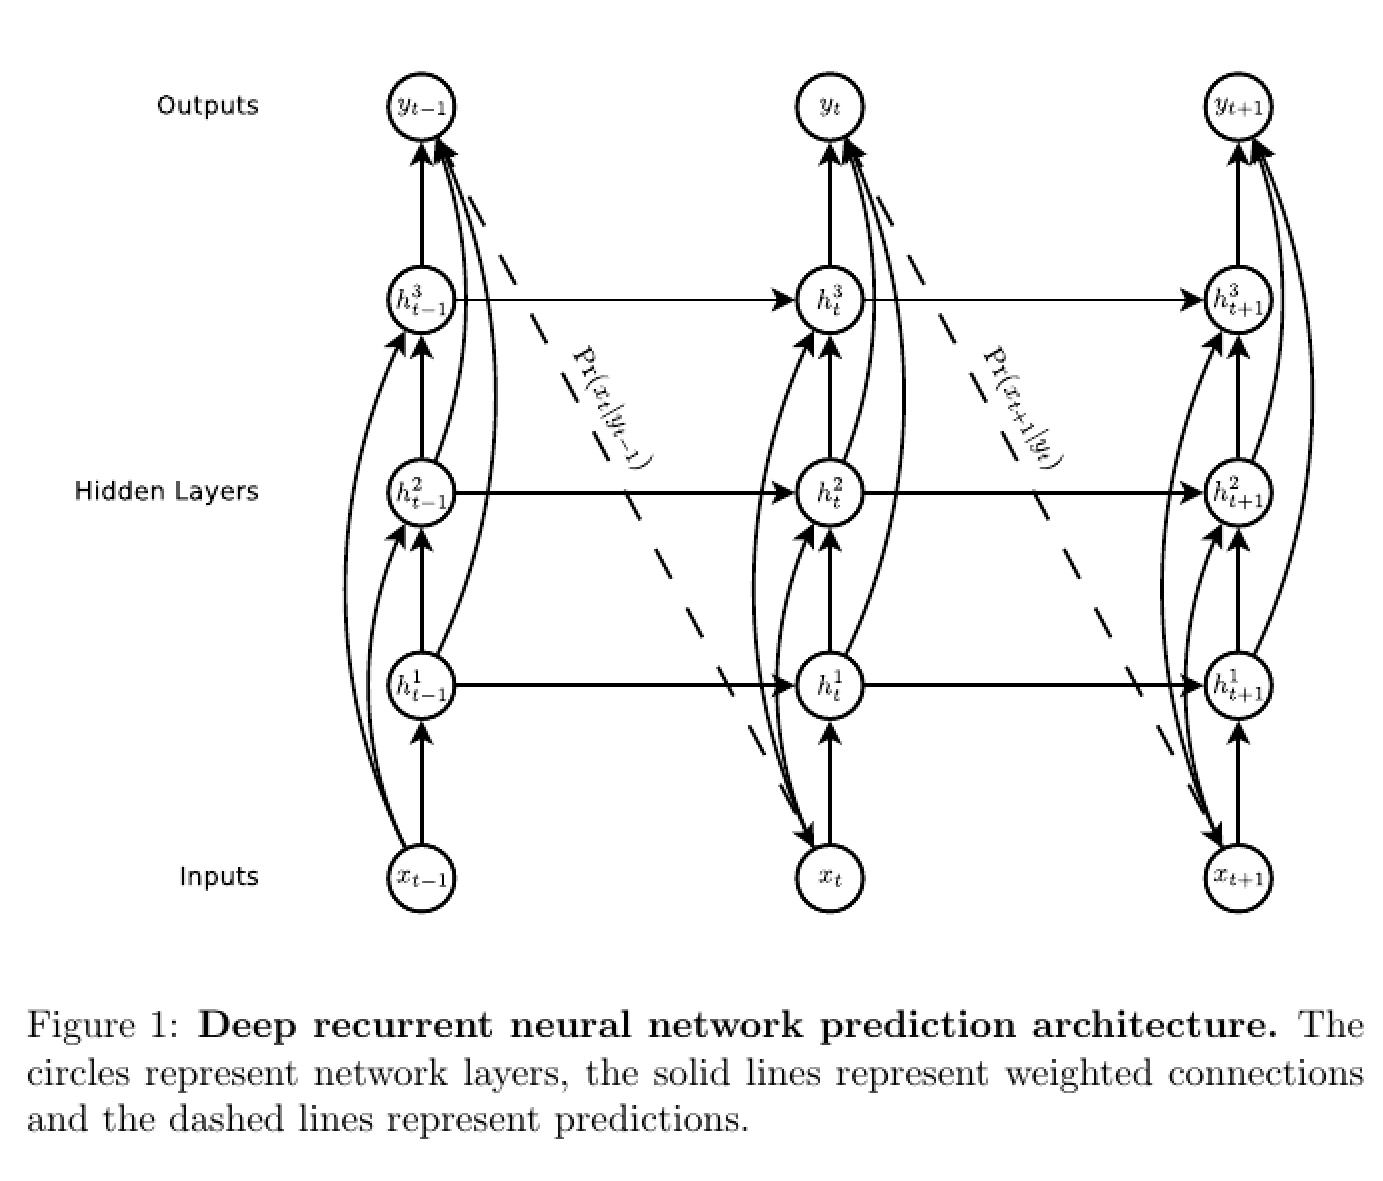
\includegraphics[width=.8\textwidth]{fig/figure1.png}
    \end{overlayarea}

    \begin{overlayarea}{\textwidth}{.3\textheight}
      \only<1>{
        Input $x_t$, hidden layers $h_t^n$, output $y_t$,
        generative model $\mathbb{P}(x_{t+1} \mid y_t)$}  
  \only<2>{
    $h_t^n = $ nonlinear link $\circ$ affine combo of $x_t$, $h_{t-1}^n$, $h_t^{n-1}$
      \begin{align*}
      h_t^n = \cH(W_{ih^n} x_t + W_{h^{n-1}h^{n}} h_{t}^{n-1} + W_{h^{n}h^{n}} h_{t-1}^n + b_h^n)
      \end{align*}
  }
  \only<3>{
    $y_t =$ nonlinear link $\circ$ affine combo of $h_t^n$
    \begin{align*}
     y_t = \mathcal{Y}(b_y + \sum_{n=1}^N W_{h^n y} h_t^n)
    \end{align*}
  }
  \only<4>{
    Train by maximizing likelihood of generative model:
    \begin{align*}
     \mathbb{P}(\mathbf{x}) &= \prod_{t=1}^T \mathbb{P}(x_t \mid y_{t-1}) 
    \end{align*}
  }
  \only<5>{
    Compute $\nabla_\Theta \log \mathbb{P}_\Theta(\bfx)$ by "truncated backpropagation through time"
    \begin{itemize}
    \item i.e., reverse chain-rule + "clip" exploding derivatives
    \end{itemize}
  }
    \end{overlayarea}
\end{frame}


\begin{frame}{Long short term memory\footnote{graphics have slight differences
      with Graves 2013; they are taken from: \\
      \url{https://colah.github.io/posts/2015-08-Understanding-LSTMs}} }
 \begin{figure}
   \centering
   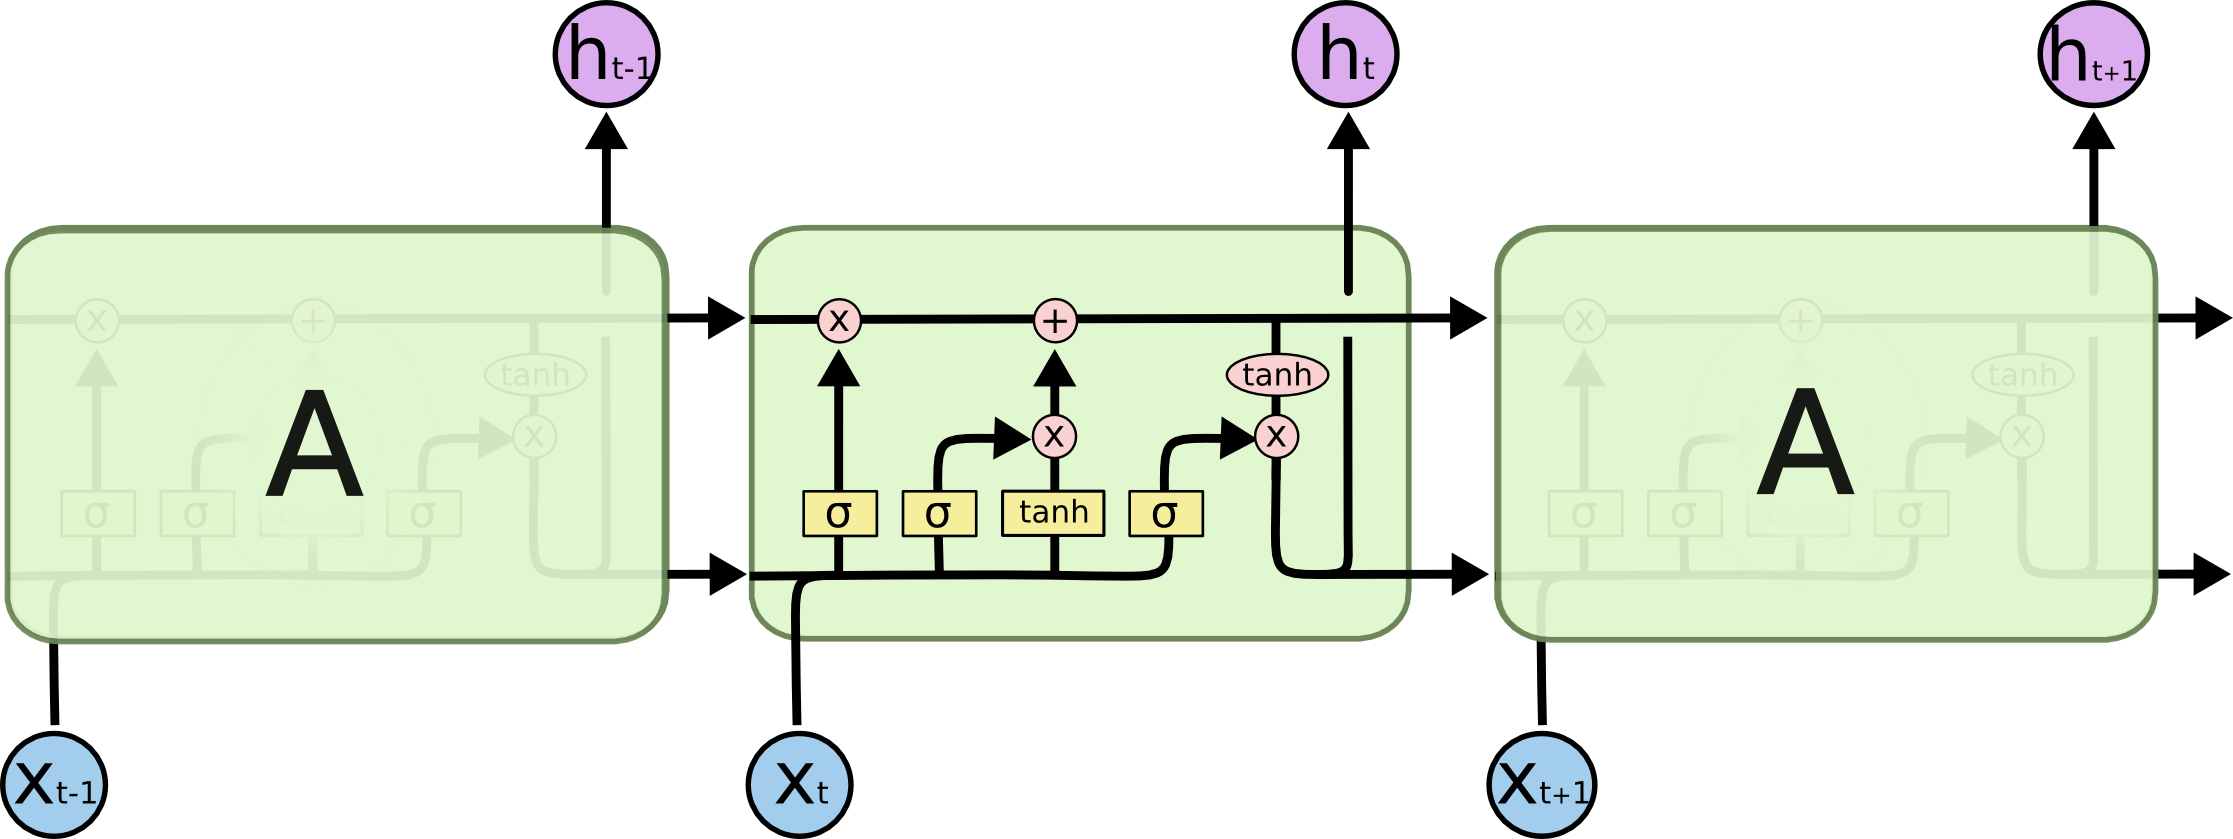
\includegraphics[width=\linewidth]{fig/LSTM3-chain.png} 
 \end{figure}
\begin{columns}
  \begin{column}{.7\textwidth}
   Information passes through a series of ``gates''
   \begin{itemize}
   \item ``Gate'' = multiplication with sigmoid
     \begin{itemize}
     \item $\sigma$ = 0 $\Rightarrow$ ``let nothing thru''
     \item $\sigma$ = 1 $\Rightarrow$ ``let all thru''
     \end{itemize}
   \end{itemize}
  \end{column}

  \begin{column}{.3\textwidth}
      \begin{figure}
        %\centering
        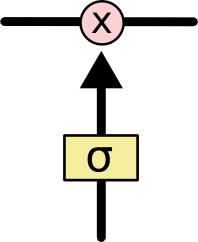
\includegraphics[width=.4\linewidth]{fig/LSTM3-gate.png} 
        \label{fig:gate}
      \end{figure}
  \end{column}
\end{columns}
\end{frame}


\begin{frame}
  \begin{overlayarea}{\textwidth}{.6\textheight}
    \begin{center}
      \only<1>{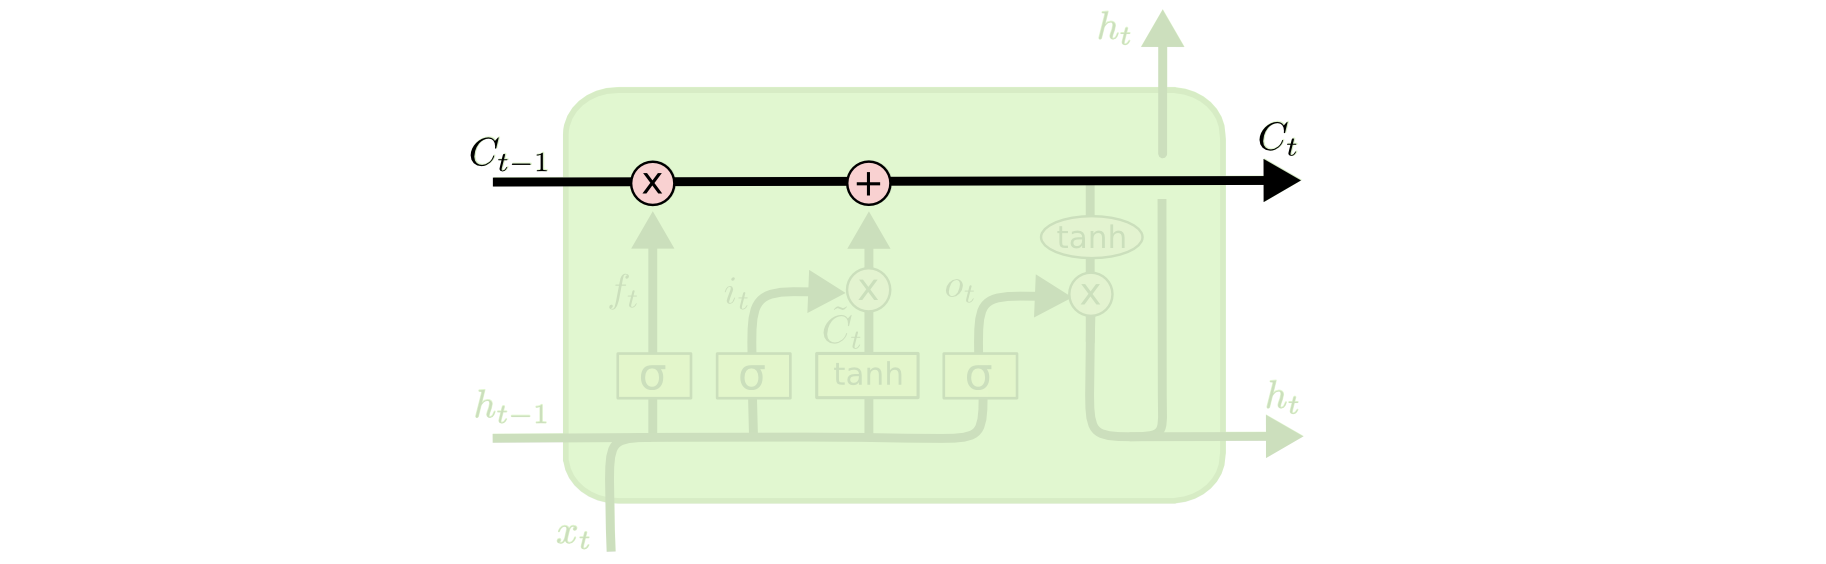
\includegraphics[width=\linewidth]{fig/LSTM3-C-line.png}} 
      \only<2>{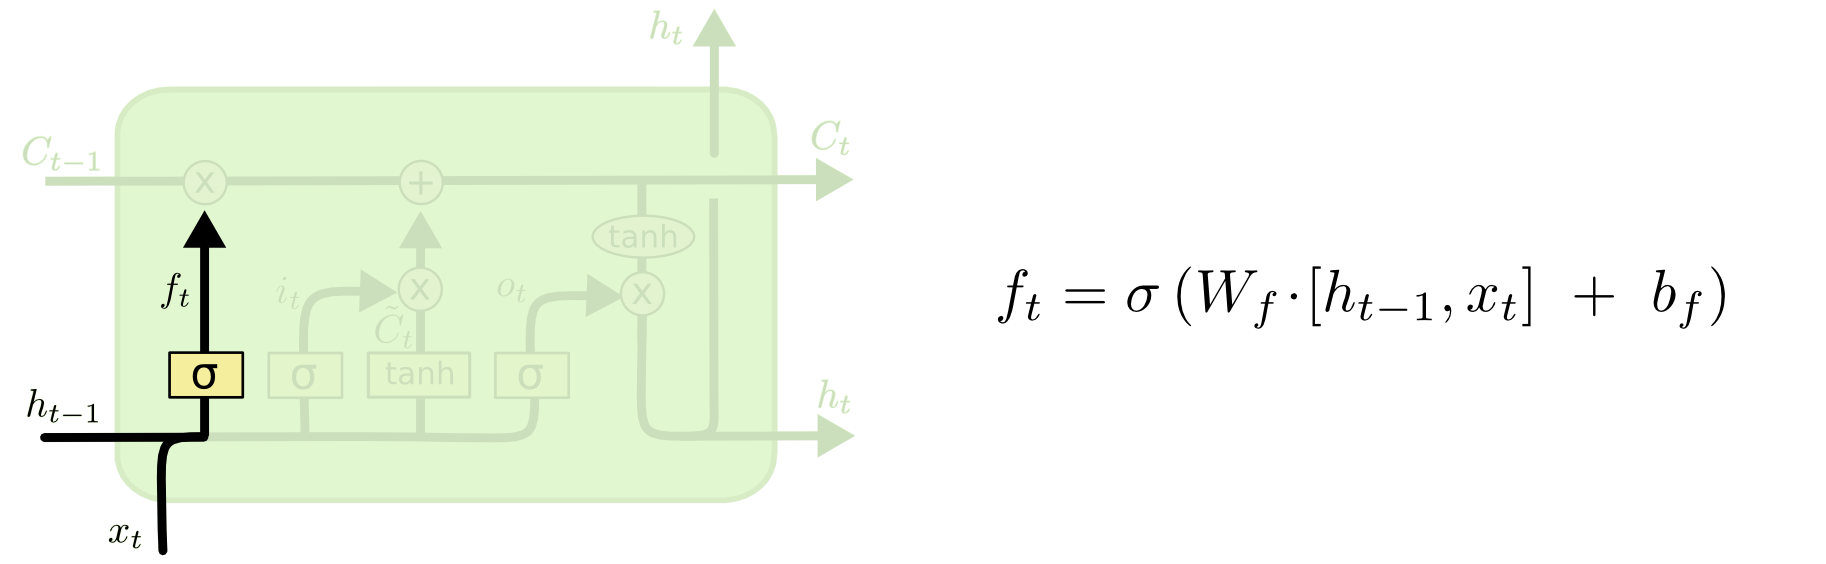
\includegraphics[width=\linewidth]{fig/LSTM3-focus-f.png}} 
      \only<3>{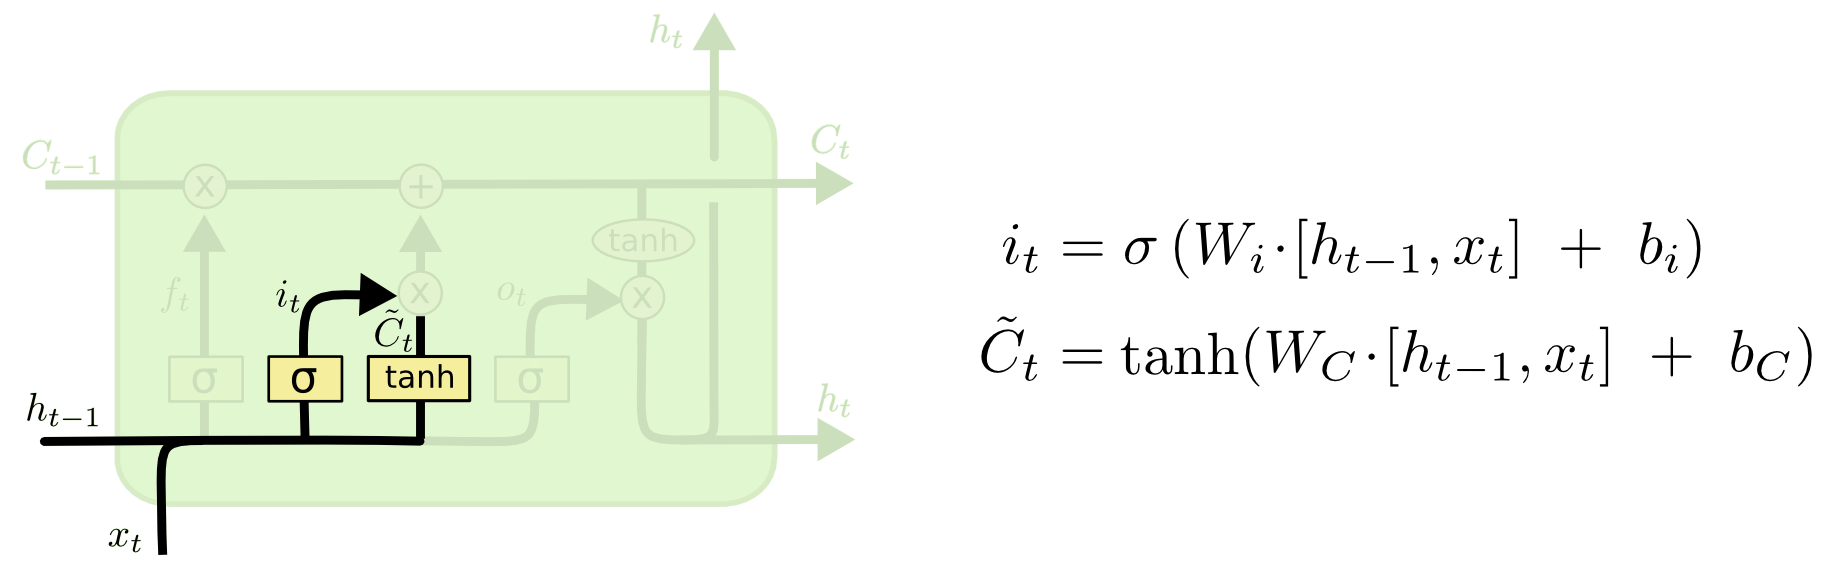
\includegraphics[width=\linewidth]{fig/LSTM3-focus-i.png}} 
      \only<4>{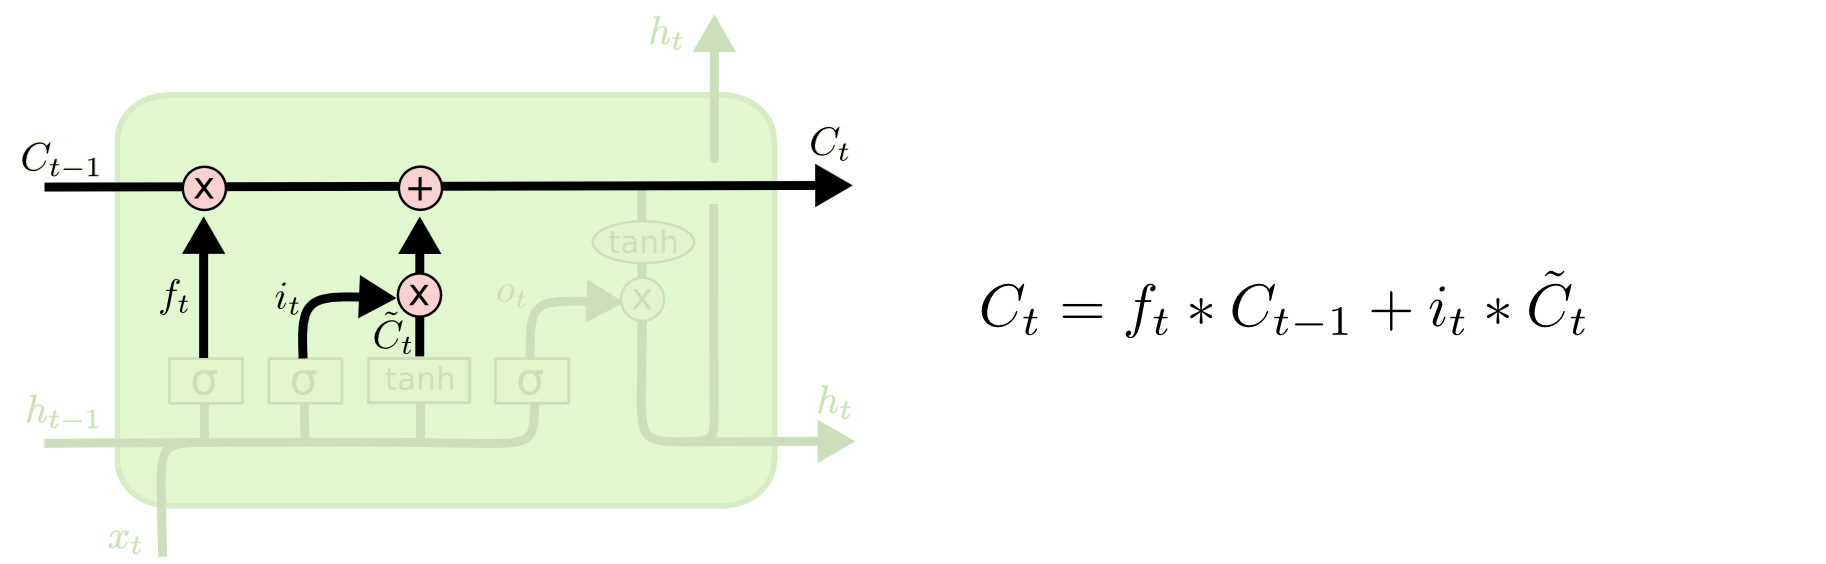
\includegraphics[width=\linewidth]{fig/LSTM3-focus-C.png}} 
      \only<5>{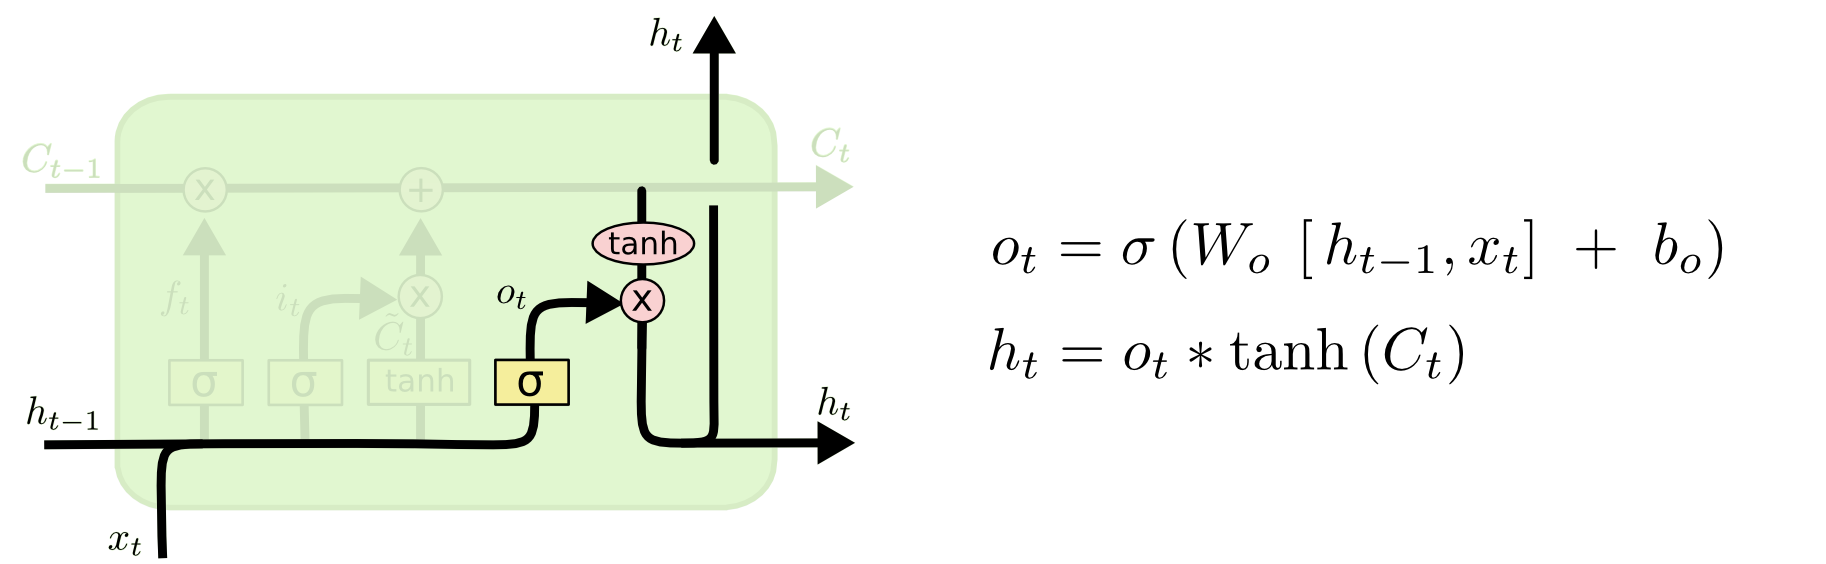
\includegraphics[width=\linewidth]{fig/LSTM3-focus-o.png}} 
    \end{center}
  \end{overlayarea}
  \only<1>{$C_t$ = ``cell state'' = flows horizontally across LSTM units}
  \only<2>{$f_t$ = ``forget gate'' = gate to forget information from $C_{t-1}$}
  \only<3>{$i_t$ = ``input gate'' = gate to add information from $h_{t-1}$ and
    $x_t$ to $C_t$}
  \only<4>{Update $C_t$ using $f_t$ and $i_t$}
  \only<5>{$o_t$ = ``output gate'' = gate to output information to cell above/right}
\end{frame}

\begin{frame}{}
  Many variations on LSTM exist. Here is the one used
  in Graves 2013:
  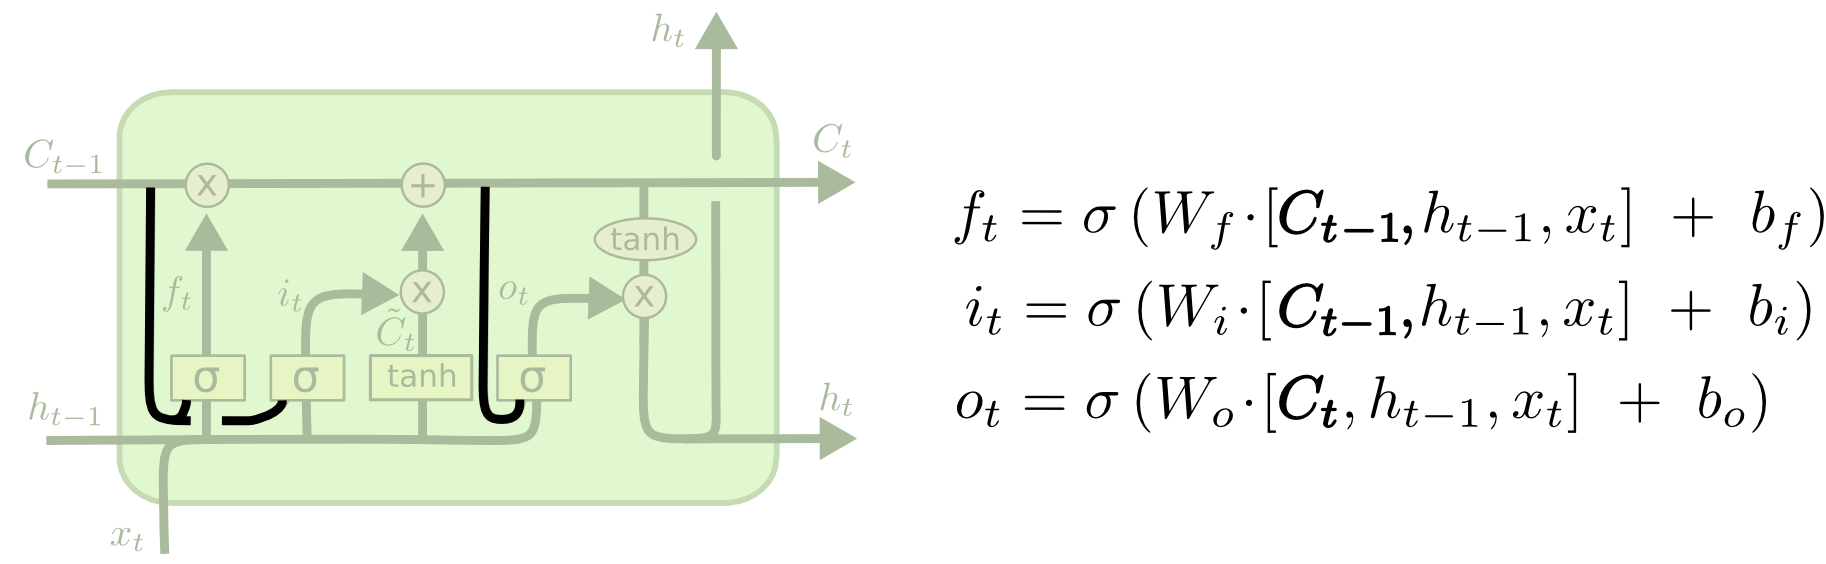
\includegraphics[width=\linewidth]{fig/LSTM3-var-peepholes.png}

  Notice the extra ``peephole'' connections from
  $C$ to $f, i, o$
\end{frame}


\section{Generating text}

\begin{frame}{Text Prediction}
  Basic framework for text prediction

  $y_t = \bbP(x_{t+1})$
  
  Per-character vs per-word prediction
\end{frame}

\begin{frame}{Penn Treebank Test Set}
  Penn Treebank
  
  Perplexity? BPC?

  Regularization schemes
\end{frame}

\begin{frame}{Wikipedia Experiments}
  \begin{itemize}
  \item   Wikipedia experiments
  \item \url{karpathy.github.io/2015/05/21/rnn-effectiveness} has some nice
    visualizations for understanding what's going on, e.g. what the inner
    neurons represent
  \end{itemize}
\end{frame}

\section{Generating handwriting}

\begin{frame}{Handwriting experiments}
  \begin{itemize}
  \item 
 Handwriting experiments 
 \item
 Mixture density outputs
 \begin{itemize}
 \item Basic framework for real valued outputs
 \end{itemize}
\item 
 Figure 10 is cool
  \end{itemize}
\end{frame}

\begin{frame}{Handwriting Synthesis}
 \begin{itemize}
 \item 
 Handwriting synthesis 
 \item Input, output sequences have different lengths
 \item Biased vs unbiased vs primed sampling
 \end{itemize}
\end{frame}

\begin{frame}{Synthesis Network}
  \begin{figure}
    \centering
  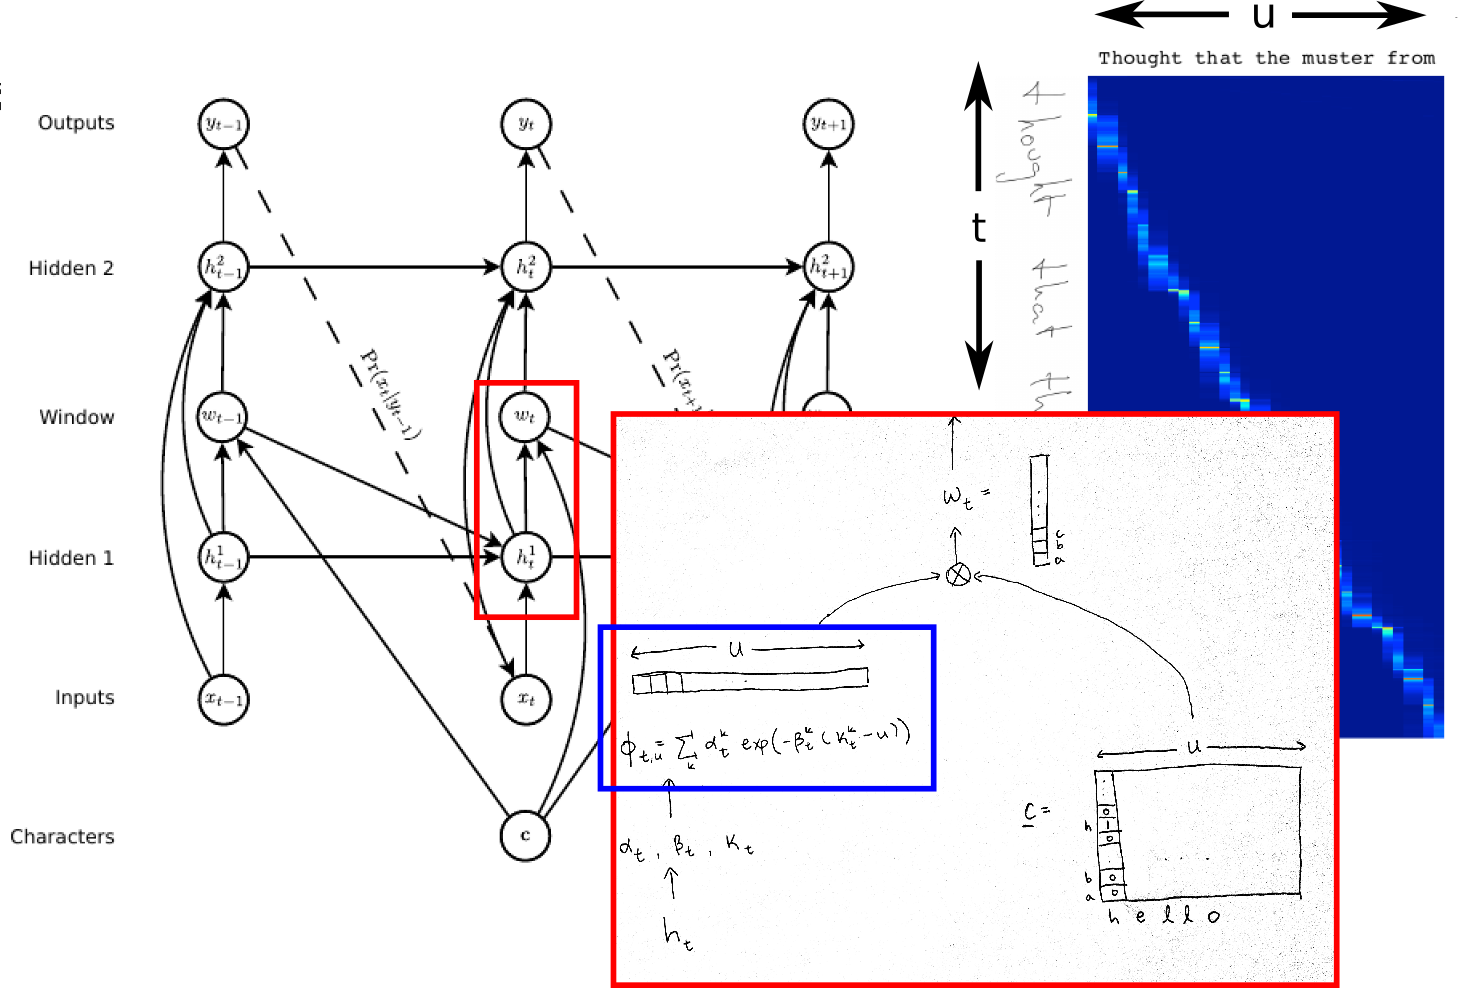
\includegraphics[width=.9\linewidth]{fig/synthesis_network3.png}
    \caption{$\phi_t(h_t^1) = $ distn over positions; $w_t = \mathbf{c}
      \phi_t =$ distn over characters}
    \label{fig:synthesis-network}
  \end{figure}
\end{frame}



\end{document}
